\documentclass[tikz,border=5mm]{standalone} 
\begin{document} 
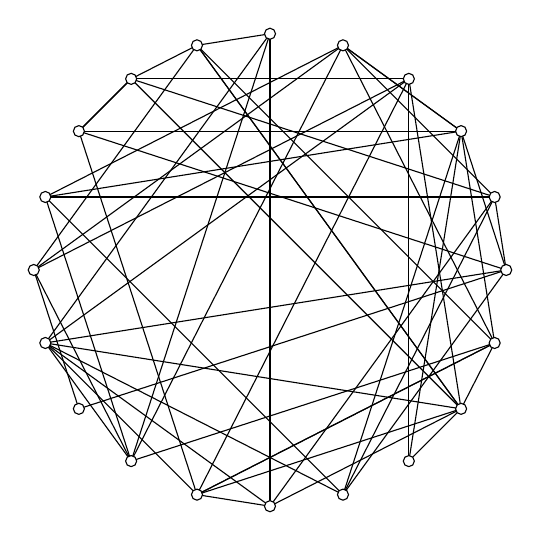
\begin{tikzpicture}
\foreach \i in {0,1,...,19}
{
  \foreach \j in {1,2,3} 
  { 
    \pgfmathsetmacro{\thenum}{int(random(0,19))}
    \draw (18*\i:3) -- (18*\thenum:3); 
  } 
} 
\foreach \i in {0,1,...,19}
{
  \filldraw [fill=white,draw=black] (18*\i:3) circle(2pt); 
} 
\end{tikzpicture} 
\end{document} 
